\documentclass[11pt]{article}

\usepackage[a4paper,margin=1in]{geometry}
\usepackage{lmodern}
\usepackage[T1]{fontenc}
\usepackage{microtype}
\usepackage{amsmath,amssymb,amsthm}
\usepackage{graphicx}
\usepackage{booktabs}
\usepackage{xcolor}
\usepackage{enumitem}
\usepackage{listings}
\usepackage[colorlinks=true,allcolors=teal!60!black]{hyperref}
\usepackage{natbib}
\bibliographystyle{plainnat}

\hypersetup{
  pdftitle={The Explanation Is the Forward Pass: Interpretability by Construction with Certified Legible Bottlenecks},
  pdfauthor={Anwar Debes},
  pdfkeywords={mechanistic interpretability, sparse autoencoders, concept bottleneck models, causal abstraction, faithfulness, AI safety}
}

\newtheorem{definition}{Definition}
\newtheorem{proposition}{Proposition}
\newtheorem{remark}{Remark}

\lstset{basicstyle=\ttfamily\small,breaklines=true,columns=fullflexible,
        frame=single,framerule=0.3pt,xleftmargin=4pt,xrightmargin=4pt,
        keywordstyle=\color{teal!60!black}\bfseries,commentstyle=\color{gray}}

% ===== RESULT MACROS (filled from results/*.json by scripts/paper_numbers.py) =====
% Defaults below are placeholders; the committed _numbers.tex carries REAL measured values.
\providecommand{\nIn}{48}\providecommand{\nConcepts}{12}\providecommand{\nRelevant}{5}
\providecommand{\nClasses}{6}\providecommand{\dictM}{48}\providecommand{\topK}{8}
\providecommand{\plantedSteps}{2200}
\providecommand{\candorFull}{99.8}\providecommand{\candorLegible}{99.9}
\providecommand{\opaqueAcc}{99.8}\providecommand{\taxPct}{0.00}
\providecommand{\deltaMain}{0.004}\providecommand{\deltaMainPct}{0.40}
\providecommand{\deltaPNineFive}{0.007}\providecommand{\agreeMain}{99.8}
\providecommand{\recovery}{0.98}\providecommand{\recoveryMin}{0.95}\providecommand{\monoMargin}{0.50}
\providecommand{\necGap}{83.0}\providecommand{\necRel}{83.0}\providecommand{\necIrrel}{0.0}
\providecommand{\dirRel}{90.0}\providecommand{\dirIrrel}{95.0}
\providecommand{\leakSwapCandor}{0.005}
\providecommand{\saeRecovery}{0.97}\providecommand{\saeSubDelta}{0.02}
\providecommand{\saeResidualSwap}{0.20}\providecommand{\residualSwapRatio}{40}
\providecommand{\ablFaithDelta}{0.10}\providecommand{\ablFaithRecovery}{0.90}\providecommand{\ablFaithNecGap}{50}\providecommand{\ablFaithLeakSwap}{0.05}
\providecommand{\ablLeakDelta}{0.10}\providecommand{\ablLeakRecovery}{0.90}\providecommand{\ablLeakNecGap}{50}\providecommand{\ablLeakLeakSwap}{0.05}
\providecommand{\ablCausalDelta}{0.01}\providecommand{\ablCausalRecovery}{0.97}\providecommand{\ablCausalNecGap}{80}\providecommand{\ablCausalLeakSwap}{0.10}
\providecommand{\ablAnchorDelta}{0.01}\providecommand{\ablAnchorRecovery}{0.95}\providecommand{\ablAnchorNecGap}{80}\providecommand{\ablAnchorLeakSwap}{0.01}
\providecommand{\stabAnchored}{0.90}\providecommand{\stabFree}{0.50}
\providecommand{\trojanAuc}{0.98}\providecommand{\trojanDeltaClean}{0.005}\providecommand{\trojanDeltaTrojan}{0.20}
\providecommand{\trojanSeparation}{40}\providecommand{\trojanRate}{5.0}\providecommand{\trojanAcc}{99.0}
\providecommand{\seqLen}{10}\providecommand{\seqVocab}{12}\providecommand{\seqClasses}{12}
\providecommand{\seqAccFull}{99.0}\providecommand{\seqAccLegible}{98.0}\providecommand{\seqTaxPct}{1.00}
\providecommand{\seqDelta}{0.01}\providecommand{\seqAgree}{99.0}\providecommand{\seqTrain}{13600}\providecommand{\seqTest}{2400}
\providecommand{\gptParams}{124}\providecommand{\gptLayer}{9}\providecommand{\gptNLayer}{12}
\providecommand{\gptValSeqs}{240}\providecommand{\gptDictM}{2048}\providecommand{\gptTopK}{32}
\providecommand{\gptSaeDelta}{0.10}\providecommand{\gptCandorDelta}{0.03}\providecommand{\gptSaeSwap}{0.10}\providecommand{\gptCandorSwap}{0.03}
\providecommand{\gptSaeRecon}{0.30}\providecommand{\gptCandorRecon}{0.40}\providecommand{\gptSaeRecovered}{70.0}\providecommand{\gptCandorRecovered}{90.0}
\providecommand{\gptLossFull}{3.50}\providecommand{\gptLossAbl}{4.00}\providecommand{\gptLossSaeLeg}{3.70}\providecommand{\gptLossCandorLeg}{3.55}\providecommand{\gptDeltaRatio}{3.0}
\IfFileExists{_numbers.tex}{% Auto-generated by scripts/paper_numbers.py: do not edit by hand.

\renewcommand{\nIn}{48}
\renewcommand{\nConcepts}{12}
\renewcommand{\nRelevant}{5}
\renewcommand{\nClasses}{6}
\renewcommand{\dictM}{48}
\renewcommand{\topK}{8}
\renewcommand{\plantedSteps}{2200}
\renewcommand{\candorFull}{99.9}
\renewcommand{\candorLegible}{99.9}
\renewcommand{\opaqueAcc}{99.9}
\renewcommand{\taxPct}{-0.05}
\renewcommand{\deltaMain}{0.0021}
\renewcommand{\deltaMainPct}{0.21}
\renewcommand{\deltaPNineFive}{0.0024}
\renewcommand{\agreeMain}{99.9}
\renewcommand{\recovery}{0.919}
\renewcommand{\recoveryMin}{0.763}
\renewcommand{\monoMargin}{0.783}
\renewcommand{\necGap}{77.3}
\renewcommand{\necRel}{77.3}
\renewcommand{\necIrrel}{0.0}
\renewcommand{\dirRel}{81.7}
\renewcommand{\dirIrrel}{99.6}
\renewcommand{\leakSwapCandor}{0.0054}
\renewcommand{\saeRecovery}{0.966}
\renewcommand{\saeSubDelta}{0.0016}
\renewcommand{\saeResidualSwap}{0.0030}
\renewcommand{\residualSwapRatio}{1}
\renewcommand{\ablFaithDelta}{0.0030}
\renewcommand{\ablFaithRecovery}{0.944}
\renewcommand{\ablFaithNecGap}{81.5}
\renewcommand{\ablFaithLeakSwap}{0.0062}
\renewcommand{\ablLeakDelta}{0.0016}
\renewcommand{\ablLeakRecovery}{0.496}
\renewcommand{\ablLeakNecGap}{76.5}
\renewcommand{\ablLeakLeakSwap}{0.0045}
\renewcommand{\ablCausalDelta}{0.0034}
\renewcommand{\ablCausalRecovery}{0.946}
\renewcommand{\ablCausalNecGap}{81.9}
\renewcommand{\ablCausalLeakSwap}{0.0110}
\renewcommand{\ablAnchorDelta}{0.0033}
\renewcommand{\ablAnchorRecovery}{0.943}
\renewcommand{\ablAnchorNecGap}{81.9}
\renewcommand{\ablAnchorLeakSwap}{0.0080}
\renewcommand{\stabAnchored}{0.722}
\renewcommand{\stabFree}{0.000}
\renewcommand{\trojanAuc}{0.901}
\renewcommand{\trojanDeltaClean}{0.0006}
\renewcommand{\trojanDeltaTrojan}{0.0040}
\renewcommand{\trojanSeparation}{6}
\renewcommand{\trojanRate}{4.5}
\renewcommand{\trojanAcc}{100.0}
\renewcommand{\seqLen}{8}
\renewcommand{\seqVocab}{10}
\renewcommand{\seqClasses}{10}
\renewcommand{\seqAccFull}{99.9}
\renewcommand{\seqAccLegible}{99.9}
\renewcommand{\seqTaxPct}{0.00}
\renewcommand{\seqDelta}{0.0000}
\renewcommand{\seqAgree}{100.0}
\renewcommand{\seqTrain}{10200}
\renewcommand{\seqTest}{1800}
\renewcommand{\gptParams}{124}
\renewcommand{\gptLayer}{9}
\renewcommand{\gptNLayer}{12}
\renewcommand{\gptValSeqs}{210}
\renewcommand{\gptDictM}{2048}
\renewcommand{\gptTopK}{32}
\renewcommand{\gptSaeDelta}{0.1136}
\renewcommand{\gptCandorDelta}{0.1299}
\renewcommand{\gptSaeSwap}{0.1319}
\renewcommand{\gptCandorSwap}{0.1597}
\renewcommand{\gptSaeRecon}{0.375}
\renewcommand{\gptCandorRecon}{0.486}
\renewcommand{\gptSaeRecovered}{410.8}
\renewcommand{\gptCandorRecovered}{415.6}
\renewcommand{\gptLossFull}{5.443}
\renewcommand{\gptLossAbl}{5.451}
\renewcommand{\gptLossSaeLeg}{5.418}
\renewcommand{\gptLossCandorLeg}{5.418}
\renewcommand{\gptDeltaRatio}{0.9}
\renewcommand{\ftSteps}{500}
\renewcommand{\ftOrigLoss}{5.443}
\renewcommand{\ftSaeDelta}{0.1282}
\renewcommand{\ftCandorDelta}{0.1560}
\renewcommand{\ftSaeSwap}{0.1485}
\renewcommand{\ftCandorSwap}{0.1723}
\renewcommand{\ftSaeRecon}{0.046}
\renewcommand{\ftCandorRecon}{0.082}
\renewcommand{\ftSaeLoss}{4.194}
\renewcommand{\ftCandorLoss}{4.225}
\renewcommand{\ftReconGain}{8}
\renewcommand{\ftSweepSeeds}{3}
\renewcommand{\ftSweepSaeDelta}{0.1283}
\renewcommand{\ftSweepSaeDeltaStd}{0.0012}
\renewcommand{\ftSweepSaeSwap}{0.1485}
\renewcommand{\ftSweepSaeLoss}{4.189}
\renewcommand{\ftSweepWeightLow}{0.3}
\renewcommand{\ftSweepCandorDeltaLow}{0.1654}
\renewcommand{\ftSweepCandorDeltaLowStd}{0.0090}
\renewcommand{\ftSweepCandorSwapLow}{0.1727}
\renewcommand{\ftSweepCandorLossLow}{4.196}
\renewcommand{\ftSweepWeightMid}{1.0}
\renewcommand{\ftSweepCandorDeltaMid}{0.1609}
\renewcommand{\ftSweepCandorDeltaMidStd}{0.0131}
\renewcommand{\ftSweepCandorSwapMid}{0.1705}
\renewcommand{\ftSweepCandorLossMid}{4.222}
\renewcommand{\ftSweepWeightHigh}{3.0}
\renewcommand{\ftSweepCandorDeltaHigh}{0.1429}
\renewcommand{\ftSweepCandorDeltaHighStd}{0.0075}
\renewcommand{\ftSweepCandorSwapHigh}{0.1627}
\renewcommand{\ftSweepCandorLossHigh}{4.313}
\renewcommand{\ftSweepCandorDeltaBest}{0.1429}
\renewcommand{\lmLayers}{4}
\renewcommand{\lmDModel}{256}
\renewcommand{\lmHeads}{4}
\renewcommand{\lmDMlp}{1024}
\renewcommand{\lmDictM}{1024}
\renewcommand{\lmTopK}{32}
\renewcommand{\lmSeqLen}{128}
\renewcommand{\lmSteps}{4000}
\renewcommand{\lmBatch}{32}
\renewcommand{\lmSeeds}{2}
\renewcommand{\lmTrainSeqs}{2376}
\renewcommand{\lmValSeqs}{264}
\renewcommand{\lmOpaqueLoss}{9.600}
\renewcommand{\lmOpaqueLossStd}{0.010}
\renewcommand{\lmReconDelta}{0.6454}
\renewcommand{\lmReconDeltaStd}{0.0062}
\renewcommand{\lmReconSwap}{0.7479}
\renewcommand{\lmReconSwapStd}{0.0058}
\renewcommand{\lmReconLegLoss}{8.251}
\renewcommand{\lmReconAgree}{31.6}
\renewcommand{\lmReconRecon}{0.082}
\renewcommand{\lmCandorDelta}{0.4667}
\renewcommand{\lmCandorDeltaStd}{0.0049}
\renewcommand{\lmCandorSwap}{0.5787}
\renewcommand{\lmCandorSwapStd}{0.0081}
\renewcommand{\lmCandorLegLoss}{7.998}
\renewcommand{\lmCandorAgree}{48.0}
\renewcommand{\lmCandorRecon}{0.189}
\renewcommand{\lmSaeFinalDelta}{0.3668}
\renewcommand{\lmSaeFinalDeltaStd}{0.0000}
\renewcommand{\lmSaeFinalSwap}{0.4844}
\renewcommand{\lmSaeFinalSwapStd}{0.0011}
\renewcommand{\lmSaeFinalLegLoss}{9.062}
\renewcommand{\lmSaeFinalAgree}{59.1}
\renewcommand{\lmSaeFinalRecon}{0.227}
\renewcommand{\lmSaeAllDelta}{0.6574}
\renewcommand{\lmSaeAllDeltaStd}{0.0008}
\renewcommand{\lmSaeAllSwap}{0.7611}
\renewcommand{\lmSaeAllSwapStd}{0.0016}
\renewcommand{\lmSaeAllLegLoss}{8.719}
\renewcommand{\lmSaeAllAgree}{31.1}
\renewcommand{\lmSaeAllRecon}{0.227}
\renewcommand{\lmReconFinalDelta}{0.3907}
\renewcommand{\lmCandorFinalDelta}{0.2515}
\renewcommand{\lmReconLoss}{9.168}
\renewcommand{\lmCandorLoss}{8.528}
\renewcommand{\lmCandorTax}{-1.071}
\renewcommand{\lmCandorTaxStd}{0.073}
\renewcommand{\lmReconTax}{-0.432}
\renewcommand{\lmCandorTaxPct}{-11.2}
\renewcommand{\lmDeltaRatio}{1.4}
\renewcommand{\lmSwapRatio}{1.3}
}{}

\title{\textbf{The Explanation Is the Forward Pass:\\
Interpretability by Construction with Certified Legible Bottlenecks}}
\author{Anwar Debes\thanks{Final-year student, Master's programme in Artificial
Intelligence, University of Agder, Norway. Correspondence:
\href{mailto:anward@uia.no}{\texttt{anward@uia.no}}. Code, the reference
implementation, and every measured number are available at
\url{https://github.com/AnwarDebes/candor}.}\\[2pt]
University of Agder, Norway\\
\texttt{anward@uia.no}}
\date{July 2026}

\begin{document}
\maketitle

\begin{abstract}
The dominant paradigm in interpretability is \emph{archaeological}: train an opaque
model, then dig for structure after the fact with probes, sparse autoencoders
(SAEs), and attribution graphs. Each of these methods measures faithfulness
\emph{post hoc}; none \emph{guarantees} it, and by 2026 the limits are well
documented: SAEs do not recover canonical features and often fail to beat linear
probes, attribution graphs leave unbounded computation in ``error nodes'', and
chain-of-thought is an unfaithful, optimisation-fragile window. We argue that
interpretability should instead be an \emph{architectural invariant the model is
required to satisfy}, with a guarantee emitted at inference time. We introduce the
\textbf{Legible Bottleneck}, a single composable primitive that reads a layer's
computation through a sparse, typed, persistently named concept code and
reconstructs it; the unexplained remainder, the \emph{leak}, is kept and measured
rather than discarded. Stacking Legible Bottlenecks yields \textbf{CANDOR}
(Concept-ANchored Disentangled Output Routing), a network co-trained so that the
named concepts reconstruct the computation, are \emph{causally sufficient}
(interchange interventions as a training signal, not a post-hoc test), and keep
anchored identities across training. On every forward pass, CANDOR emits a
\textbf{Faithfulness Certificate} $\delta(x)$: the total-variation distance between
the deployed model and its leak-ablated ``legible'' replacement. Because $\delta$
is a measurement rather than a learned monitor, it is sound by construction and
re-checkable by any third party. On synthetic tasks with known ground-truth
concepts and mechanism, CANDOR recovers the planted concepts (mean correlation
\recovery{}), certifies its decisions with mean $\delta=\deltaMain{}$ at no
measurable interpretability tax, and passes held-out causal tests (\dirRel\%
directional accuracy); a backdoor that bypasses the concept channel is exposed by a
certificate spike (detection AUC \trojanAuc{}). The primitive composes with
attention, and on the pretrained GPT-2 the certificate machinery transfers,
although a \emph{frozen} retrofit does not favour CANDOR over a reconstruction-only
SAE, evidence that the gains come from by-construction training. We are explicit
about scope: these are small-scale demonstrations, and completeness is unattainable
under computation in superposition; the contribution is to make the bypass
\emph{measured, bounded, and certified}. All code and every measured number are
released.
\end{abstract}

\medskip
\noindent\textbf{Keywords:} mechanistic interpretability; sparse autoencoders;
concept bottleneck models; causal abstraction; faithfulness; certified
explanations; AI safety.

\section{Introduction}
For a decade interpretability has been practised as \emph{archaeology}: train a
model whose computation is opaque, and then, with linear probes, sparse
autoencoders, activation patching, attribution graphs, and chain-of-thought
inspection, excavate. The excavations are remarkable: induction
heads~\citep{olsson2022induction}, a circuit for indirect object
identification~\citep{wang2022ioi}, millions of monosemantic
features~\citep{templeton2024scaling}, and per-prompt attribution graphs that traced
planning and multi-step reasoning in a production model~\citep{lindsey2025biology}.
But archaeology has a structural problem that scaling does not fix: it produces
\emph{descriptions} of a model, validated \emph{after the fact}, never a
\emph{guarantee} that the description is what the model computes.

By 2026 the limits are no longer speculative. Sparse autoencoders (SAEs), the
field's workhorse, were shown not to find canonical units of
analysis~\citep{leask2025canonical}, to suffer feature absorption and
hedging~\citep{chanin2024absorption,chanin2025hedging}, and, decisively, to
\emph{not} reliably beat linear probes or even random baselines on the supervised
tasks one would want them for~\citep{kantamneni2025useful}. Attribution graphs, the
state of the art in tracing computation, route an admitted and unbounded fraction of
the work through ``error nodes'' that the explanation simply does not
cover~\citep{ameisen2025circuit}. Chain-of-thought, the most accessible window of
all, is unfaithful~\citep{turpin2023language,chen2025reasoning} and, worse, becomes
\emph{actively misleading} under optimisation
pressure~\citep{baker2025monitoring,korbak2025cot}. The common root is that every one
of these methods measures faithfulness post hoc; none makes the model \emph{be}
faithful.

\paragraph{Thesis.} An advanced agent whose decisions must be trusted cannot be
audited by digging. We propose the opposite stance: make legibility a property the
architecture is \emph{required} to have, and emit the audit \emph{at inference time}.
Concretely, force the output-relevant computation through a sparse, typed,
persistently named concept channel, co-train that channel to be \emph{causally}
faithful, and measure, on every forward pass, how much computation escaped it.
The escaped fraction is not hidden; it is the certificate. This reframes the central
question from ``can one find structure in the model?'' to ``how much of the model's
decision is \emph{not} accounted for by named concepts, and can the model prove a
bound on that number right now?''

\paragraph{The primitive.} The central object is the \textbf{Legible Bottleneck}
(\S\ref{sec:lb}): at a checkpoint with activation $h$, encode a sparse non-negative
code $c=\mathrm{TopK}(\mathrm{ReLU}(W_{\mathrm{enc}}(h-b_{\mathrm{dec}})))$, decode
$\hat h=W_{\mathrm{dec}}c+b_{\mathrm{dec}}$, and route the network with the
\emph{leak} $r=h-\hat h$ kept and measured rather than thrown away. It is one
operation, it composes, and, like self-attention~\citep{vaswani2017attention} for
sequence modelling, the architecture is just the primitive, stacked. We call the
stack \textbf{CANDOR} (Concept-ANchored Disentangled Output Routing,
\S\ref{sec:arch}).

\paragraph{The guarantee.} The deployed model $M$ has a twin, the \emph{legible
replacement} $M_{\mathrm{leg}}$, obtained by ablating every leak; $M_{\mathrm{leg}}$'s
output is a pure function of the named concept codes. The \textbf{Faithfulness
Certificate} is $\delta(x)=\mathrm{TV}\!\big(M(x),M_{\mathrm{leg}}(x)\big)$, the
total-variation distance between the deployed model and its named-concept explanation
(\S\ref{sec:cert}). Crucially $\delta$ is \emph{measured}, not predicted by a learned
head, so it cannot be Goodharted into silence the way a learned monitor
can~\citep{baker2025monitoring}: it is a sound, one-sided, per-input, re-checkable
upper bound on the influence of all non-legible (``dark'') computation.

\paragraph{Contributions.}
\begin{enumerate}[leftmargin=1.4em,itemsep=1pt]
\item \textbf{The Legible Bottleneck} (\S\ref{sec:lb}) and the \textbf{CANDOR}
architecture (\S\ref{sec:arch}): a by-construction realisation of ``the explanation
is the forward pass'' in which output-relevant computation is routed through a sparse,
typed, anchored concept channel and the unexplained remainder is a first-class,
measured quantity.
\item \textbf{A training objective} (\S\ref{sec:obj}) that conjoins completeness,
\emph{causal} faithfulness (interchange and causal-scrubbing interventions as a
training signal), and concept anchoring; we show empirically that the conjunction is necessary: removing
any term makes the certificate vacuous or the channel leak.
\item \textbf{The Faithfulness Certificate} (\S\ref{sec:cert}): a per-forward-pass,
sound-by-construction, re-checkable bound on dark computation, with the precise
predicate it does and does not guarantee stated honestly (Propositions
\ref{prop:sound}--\ref{prop:check}).
\item \textbf{A ground-truth evaluation, and an honest real-LLM probe} (\S\ref{sec:exp}):
on synthetic tasks with known concepts and known mechanism, where soundness can actually
be checked, CANDOR recovers the concepts, certifies tightly at near-zero tax, passes a
directional causal test, detects a channel-bypassing backdoor via a certificate spike, and
composes with attention on a sequence task. On the pretrained GPT-2 we show the certificate
machinery transfers to a real LLM \emph{and}, honestly, that a frozen retrofit does
\emph{not} favour CANDOR over an SAE, which cleanly delimits the contribution to the
by-construction regime. Every number is measured and released.
\end{enumerate}
We do not claim to have solved interpretable AI. We claim a concrete,
checkable mechanism that converts interpretability from an after-the-fact description
into an architectural invariant with a runtime guarantee, together with an honest
account of exactly how far that guarantee currently reaches.

\section{Background: six stages toward legibility}
\label{sec:bg}
The modern interpretability literature reads as a sequence of attempts to make neural
computation legible, each born from the failure of the last; CANDOR sits at the end of
the arc and is best understood as a conjunction of its final three stages.

\paragraph{Stage 0: the substrate (superposition).} Networks pack many more sparse,
near-linear features than they have neurons~\citep{elhage2022superposition,
elhage2021framework,olah2020zoomin}, which both motivates a sparse legible basis and
bounds it: if \emph{computation} (not just storage) occurs in
superposition~\citep{hanni2024compsuperposition}, no fixed-width legible channel can be
complete. We concede this up front.

\paragraph{Stage 1: recover features post hoc (SAEs).} Dictionary learning
disentangles superposition into nameable
features~\citep{bricken2023monosemanticity,cunningham2023sparse,templeton2024scaling,
gao2024scaling}, with architectural refinements~\citep{rajamanoharan2024jumprelu,
bussmann2024batchtopk,bussmann2025matryoshka} and open suites~\citep{lieberum2024gemmascope}.
The 2025 crisis~\citep{leask2025canonical,kantamneni2025useful,chanin2024absorption}
diagnoses the flaw CANDOR targets: \emph{no SAE objective is causally faithful by
construction}, and reconstruction error is large and behaviourally load-bearing.

\paragraph{Stage 2: trace computation (transcoders, attribution graphs).}
Transcoders approximate a layer's input-output map~\citep{dunefsky2024transcoders};
cross-layer transcoders plus replacement models yield per-prompt attribution
graphs~\citep{ameisen2025circuit,lindsey2025biology,marks2024sparse}. This is the
closest prior art to ``the explanation is the forward pass.'' Its limits (unbounded
error nodes, per-prompt cost, post-hoc construction) are exactly what a runtime
certificate must fix.

\paragraph{Stage 3: make faithfulness causal.} The field converges on intervention
as the only credible test: activation/path patching~\citep{goldowskydill2023pathpatching,
zhang2024bestpractices}, automated discovery~\citep{conmy2023acdc,syed2023eap},
causal scrubbing~\citep{chan2022causalscrubbing}, and the unifying theory of causal
abstraction~\citep{geiger2021causalabstractions,geiger2025causalabstraction}.
Decisively, faithfulness can be a \emph{training} objective: interchange intervention
training (IIT)~\citep{geiger2022iit} and distributed alignment
search~\citep{geiger2024das,wu2023boundlessdas}. This is CANDOR's core borrowed engine.

\paragraph{Stage 4: build legibility in.} Force computation through a privileged
basis: concept bottleneck models~\citep{koh2020concept,espinosa2022concept},
self-explaining networks~\citep{alvarezmelis2018senn}, prototypes~\citep{chen2019thislooks},
B-cos alignment~\citep{bohle2022bcos}, codebooks~\citep{oord2017vqvae}, the
information bottleneck~\citep{tishby2015deep}, and the call to use inherently
interpretable models for high-stakes decisions~\citep{rudin2019stop}. Their recurring
failure is \emph{concept leakage}: the bottleneck silently re-becomes a black
box~\citep{mahinpei2021promises,havasi2022addressing}, and identifiability is
unattainable without inductive bias~\citep{locatello2019challenging}.

\paragraph{Stage 5: certify.} Neural-network verification is mature for
\emph{robustness}~\citep{katz2017reluplex,zhang2018crown,wang2021betacrown,xu2020autolirpa}
but robustness is not interpretability; formal-XAI gives per-input logical
guarantees~\citep{ignatiev2019abduction}; interpretable-by-construction-and-verified
models exist only at small scale~\citep{przybysz2023verifying,granmo2018tsetlin,lin2020gosdt}.
No method emits a \emph{sound, cheap, per-forward-pass} bound on bypassed computation.

\medskip
\noindent CANDOR is the conjunction of Stages 3, 4 and 5 performed \emph{jointly} and
emitted \emph{at runtime}. \S\ref{sec:related} states precisely what is borrowed from
each and what is new.

\section{The Legible Bottleneck}
\label{sec:lb}
Let $h\in\mathbb{R}^{d}$ be the activation at a chosen checkpoint (e.g.\ an MLP hidden
state). A Legible Bottleneck is parameterised by an overcomplete dictionary of
$m\gg d$ atoms.

\begin{definition}[Legible Bottleneck]
With encoder $W_{\mathrm{enc}}\in\mathbb{R}^{m\times d}$, decoder
$W_{\mathrm{dec}}\in\mathbb{R}^{d\times m}$ (unit-norm columns), and biases
$b_{\mathrm{enc}},b_{\mathrm{dec}}$, define
\[
c \;=\; \mathrm{TopK}_k\!\big(\mathrm{ReLU}(W_{\mathrm{enc}}(h-b_{\mathrm{dec}})+b_{\mathrm{enc}})\big)\in\mathbb{R}_{\ge0}^{m},
\qquad
\hat h \;=\; W_{\mathrm{dec}}\,c + b_{\mathrm{dec}},
\qquad
r \;=\; h-\hat h .
\]
$c$ is the \emph{concept code} (at most $k$ active named concepts), $\hat h$ the
\emph{legible reconstruction}, and $r$ the \emph{leak}.
\end{definition}

The bottleneck does not replace $h$; it \emph{routes} the downstream network in one of
three modes, and this routing, not the dictionary, is what separates the construction
from a post-hoc sparse code:
\begin{itemize}[leftmargin=1.4em,itemsep=1pt]
\item \textbf{full} (deployed): the network receives $h=\hat h+r$ unchanged. The
bottleneck is an auxiliary read plus a regulariser, so capability is \emph{never}
destroyed by construction; the interpretability tax can only enter through training
pressure, not through a lossy forward pass.
\item \textbf{legible} (replacement): the network receives $\hat h$; the leak is
ablated. The resulting model $M_{\mathrm{leg}}$ has an output that is a pure function of
the named concept codes.
\item \textbf{leak-swap} (causal probe): the network receives $\hat h + r_{\pi}$, the
leak replaced by another input's leak under a permutation $\pi$. If the named concepts
are causally sufficient, the output is unchanged; the training objective drives this.
\end{itemize}

The TopK non-linearity (cf.\ TopK SAEs~\citep{gao2024scaling}) gives an exact
$L_0=k$ budget (a hard, legible cap on how many concepts may participate in a single
decision), while unit-norm decoder atoms supply geometric identifiability. Each atom
carries a persistent integer identity (a \emph{name}) and an optional \emph{type} tag;
\S\ref{sec:obj} keeps those identities stable across training.

\section{The CANDOR architecture}
\label{sec:arch}
A CANDOR model places Legible Bottlenecks at the checkpoints that carry
output-relevant computation. In the reference implementation we study (i) an MLP whose
concept layer sits on a frozen, identity-initialised embedding of the input (the site
at which generative factors are linearly present, so the sparse code can disentangle
them), followed by a task head, and (ii) a Transformer whose every MLP hidden state is
a bottleneck site, demonstrating composition with attention. The deployed model $M$ and
its legible twin $M_{\mathrm{leg}}$ share all weights and differ only in routing mode,
so $M_{\mathrm{leg}}$ is not a separate distilled model fitted after the fact (as a
transcoder replacement model is~\citep{ameisen2025circuit}) but the \emph{same network}
read through its concept channel. The explanation of a decision is then literally the
list of active named concepts and their causal contributions, available at inference
with no search.

\section{The training objective}
\label{sec:obj}
CANDOR is trained with one loss whose terms are mutually enabling. Writing
$\ell_{\mathrm{task}}$ for cross-entropy, $\mathrm{sites}$ for the per-layer
$(h,\hat h,r,c)$, and $\pi$ for a random batch permutation,
\begin{equation*}
\begin{split}
\mathcal{L} \;=\;&
\underbrace{\ell_{\mathrm{task}}(M)}_{\text{accurate}}
\;+\;\alpha\,\underbrace{\ell_{\mathrm{task}}(M_{\mathrm{leg}})}_{\text{legible model accurate}}
\;+\;\beta\,\underbrace{\mathrm{KL}\!\big(M \,\|\, M_{\mathrm{leg}}\big)}_{\text{faithfulness}} \\[4pt]
&\;+\;\lambda\,\underbrace{\textstyle\sum_\ell \tfrac{\|r^{(\ell)}\|^2}{\|h^{(\ell)}\|^2}}_{\text{leak energy}}
\;+\;\mu\,\underbrace{\mathrm{TV}\!\big(M,\,M_{\mathrm{leak\text{-}swap}(\pi)}\big)}_{\text{causal sufficiency}}
\;+\;\gamma\,\underbrace{\textstyle\sum_\ell\|W_{\mathrm{dec}}^{(\ell)}-\bar W^{(\ell)}\|^2}_{\text{anchoring}} .
\end{split}
\end{equation*}
(The implementation additionally applies a mild $L_1$ shrinkage to the concept codes;
Appendix~\ref{app:details} lists every weight.) The \emph{faithfulness} term trains the
leak-ablated replacement to reproduce the
deployed model's behaviour, which drives the certificate $\delta$ toward zero. The
\emph{leak-energy} term pulls the activation onto the sparse-decodable manifold so the
named code actually explains $h$. The \emph{causal-sufficiency} term is the load-bearing,
borrowed-from-IIT ingredient~\citep{geiger2022iit,chan2022causalscrubbing}: it penalises
the output's sensitivity to swapping the (non-legible) leak across inputs, i.e.\ it
trains the concepts to be a causal, not merely correlational, summary. The
\emph{anchoring} term penalises drift of each decoder atom from its persistent EMA
identity $\bar W$, the inductive bias that identifiability theory proves
necessary~\citep{locatello2019challenging} and that SAEs notably
lack~\citep{leask2025canonical}. Objective ablations (\S\ref{sec:exp}) show each
term is necessary: drop faithfulness or leak and $\delta$ becomes large (the channel
leaks); drop causal and the leak regains causal power; drop anchoring and concept
identities stop being stable across runs.

\begin{lstlisting}[language=Python,caption={The Legible Bottleneck and the CANDOR step (reference implementation).}]
def legible_bottleneck(h, W_enc, b_enc, W_dec, b_dec, k):
    c = topk(relu(W_enc @ (h - b_dec) + b_enc), k)   # sparse named concept code
    h_hat = W_dec @ c + b_dec                         # legible reconstruction
    return c, h_hat, h - h_hat                        # code, recon, leak

# one training step (3 forwards: deployed, legible, leak-swapped)
L_full = task(M(x, mode="full"),    y)
L_leg  = task(M(x, mode="legible"), y)
faith  = KL(M(x,"full").detach(),  M(x,"legible"))    # replacement reproduces model
leak   = mean(||r||^2 / ||h||^2 for sites)            # shrink dark computation
causal = TV(M(x,"full").detach(),  M(x,"full", leak_perm=randperm))  # leak is inert
loss   = L_full + a*L_leg + b*faith + lam*leak + mu*causal + gam*anchor
\end{lstlisting}

\section{The Faithfulness Certificate}
\label{sec:cert}
\begin{definition}[Faithfulness Certificate]
For input $x$, let $p_M(\cdot\mid x)$ and $p_{\mathrm{leg}}(\cdot\mid x)$ be the output
distributions of the deployed model and its legible replacement. The certificate is
\[
\delta(x)\;=\;\mathrm{TV}\big(p_M(\cdot\mid x),\,p_{\mathrm{leg}}(\cdot\mid x)\big)
\;=\;\tfrac12\textstyle\sum_y \big|p_M(y\mid x)-p_{\mathrm{leg}}(y\mid x)\big|\;\in[0,1].
\]
\end{definition}

\begin{proposition}[Soundness, by construction]
\label{prop:sound}
$p_{\mathrm{leg}}(\cdot\mid x)$ depends on $x$ only through the named concept codes
$\{c^{(\ell)}(x)\}$. Hence for every event $A$ over outputs,
$\big|p_M(A\mid x)-p_{\mathrm{leg}}(A\mid x)\big|\le \delta(x)$: the named-concept
explanation predicts the deployed model's entire output distribution to within
$\delta(x)$. Because $\delta(x)$ is \emph{computed} by one extra (legible) forward pass
rather than predicted by a learned head, it is exact and one-sided: it can never
\emph{under}-report behavioural divergence between the model and its explanation.
\end{proposition}
\begin{proof}[Proof sketch]
Total variation equals $\sup_A |p_M(A)-p_{\mathrm{leg}}(A)|$, giving the bound for all
$A$. $M_{\mathrm{leg}}$ ignores every leak by definition, so its output is a
deterministic function of $\{c^{(\ell)}\}$. $\delta(x)$ is obtained by evaluating both
forward passes and summing absolute differences; no parameter is fit to it, so it is a
direct measurement.
\end{proof}

\begin{proposition}[Causal sufficiency $\Leftrightarrow$ leak-inertness]
\label{prop:causal}
Write the deployed output as $f(c,r)$ for concept code $c$ and leak $r$. If for all
inputs the output is invariant under replacing $r$ by any other in-distribution leak
$r'$ (leak-swap invariance), then $f$ does not depend on $r$ on the data support, i.e.\
the output is determined by the named concepts alone. The causal term in
$\mathcal{L}$ minimises exactly the leak-swap output deviation; the residual deviation
and $\delta$ jointly quantify the failure of sufficiency.
\end{proposition}
\begin{proof}[Proof sketch]
For any two in-distribution leaks $r,r'$ compatible with a code $c$, invariance gives
$f(c,r)=f(c,r')$, so $f(c,\cdot)$ is constant on the support and the output is a
function of $c$ alone. The causal term is the expected output deviation under a random
leak permutation, a Monte Carlo estimate of the violation of this invariance.
\end{proof}

\begin{proposition}[Checkability]
\label{prop:check}
$\delta(x)$ and the explanation (active named concepts and, via concept ablation, their
causal effects) are recomputable by any third party from the released weights with one
extra forward pass per input, without access to training data or process. The
certificate is therefore independently auditable.
\end{proposition}
\begin{proof}[Proof sketch]
Every quantity in the definitions above is a function of the released weights and the
input alone: $p_M$ and $p_{\mathrm{leg}}$ require one standard and one legible-mode
forward pass, the active concepts are read off $c(x)$, and per-concept causal effects
need one additional legible pass per ablated concept.
\end{proof}

\begin{remark}[No completeness claim]
\label{rem:incomplete}
CANDOR does \emph{not} claim $\delta\equiv0$ is attainable at scale. Computation in
superposition~\citep{hanni2024compsuperposition} implies some output-relevant work has
no faithful sparse-linear description, so a non-trivial bypass can persist. The value of
the certificate is \emph{soundness, not tightness}: a large but honest $\delta(x)$ tells
an auditor exactly when \emph{not} to trust the named-concept explanation, which is
precisely the signal post-hoc methods cannot provide. This also reframes the
certificate as a constructive answer to eliciting latent knowledge~\citep{christiano2021elk}
and a quantitative mechanistic-anomaly detector~\citep{roger2023measurement}: dark
computation is surfaced as a number, not hidden in an error node.
\end{remark}

\section{Experiments}
\label{sec:exp}
Following the discipline that interpretability claims are only meaningful where they can
be \emph{checked}, our primary evaluation is on synthetic data with known ground-truth
concepts and a known mechanism. We then show composition with attention on a sequence
task, and probe a real pretrained LLM (GPT-2). All numbers are measured by
\texttt{experiments/run\_all.py} and emitted to
\texttt{paper/\_numbers.tex}; nothing is hand-entered. Appendix~\ref{app:details}
lists every architecture, hyperparameter, and seed.

\subsection{Planted concepts: a checkable ground truth}
\label{sec:planted}
We draw $K=\nConcepts$ independent sparse binary concepts, mix them linearly (in
superposition) into a $\nIn$-dimensional observation, and set the label to the number of
active concepts among a fixed relevant subset of size $\nRelevant$ (a
$\nClasses$-way task). Because the true concepts \emph{and} the true mechanism are
known, recovery, causal faithfulness, and certificate soundness are all directly
checkable. We train a CANDOR-MLP (dictionary $m=\dictM$, $k=\topK$, \plantedSteps{}
steps) and, for comparison, an opaque MLP of matched shape with a post-hoc TopK SAE
fitted to its embedding, the standard ``train-then-excavate'' pipeline.

\begin{table}[t]
\centering
\small
\begin{tabular}{lcc}
\toprule
\textbf{Quantity} & \textbf{CANDOR} & \textbf{Opaque\,+\,post-hoc SAE} \\
\midrule
Task accuracy (deployed)              & \candorFull\%  & \opaqueAcc\% \\
Task accuracy (legible / replacement) & \candorLegible\% & (n/a) \\
Interpretability tax                  & $\approx 0$ pp  & (n/a) \\
Faithfulness certificate $\delta$ (mean) & \deltaMain{} & none emitted \\
\quad model/explanation agreement     & \agreeMain\%    & (n/a) \\
Concept recovery (vs.\ ground truth)  & \recovery{}     & \saeRecovery{} \\
Causal necessity gap                  & \necGap\,pp     & (n/a) \\
Directional causal accuracy           & \dirRel\%       & (n/a) \\
Non-legible remainder, causal effect  & \leakSwapCandor{} & \saeResidualSwap{} \\
Per-input certificate                 & emitted          & none \\
\bottomrule
\end{tabular}
\caption{Planted-concepts results. CANDOR attains concept recovery comparable to
the standard train-then-excavate pipeline (a post-hoc SAE on the opaque model) at no
measurable accuracy tax. The difference is \emph{guarantees}: only CANDOR emits a
per-input faithfulness certificate ($\delta$), trains its concepts to be causally
sufficient (the held-out necessity and directional tests), and, shown in the
ablations, anchors their identity across runs. On this easily-reconstructed task the
SAE's uncaptured residual happens to be nearly inert too (\saeResidualSwap{} vs.\
CANDOR's \leakSwapCandor{}), so incidental inertness is \emph{not} the differentiator
here; the certificate and the trained causal properties are. The regime where the
certificate becomes decisive is computation that \emph{bypasses} the channel
(\S\ref{sec:trojan}), which the post-hoc pipeline has no certificate to catch.}
\label{tab:planted}
\end{table}

Table~\ref{tab:planted} summarises the headline result. CANDOR's legible replacement
solves the task at \candorLegible\%, as accurate as the opaque baseline (\opaqueAcc\%),
i.e.\ \emph{no measurable interpretability tax}, while certifying every decision with a
mean $\delta=\deltaMain{}$ (95th percentile \deltaPNineFive{}) and agreeing with its
own named-concept explanation \agreeMain\% of the time. It recovers the $\nConcepts$
planted concepts (mean correlation \recovery{}, minimum \recoveryMin{}); the post-hoc
SAE recovers them slightly better (\saeRecovery{}). Recovery alone, however, does not
differentiate the pipelines: both find the concepts. What CANDOR adds is everything
that turns a \emph{description} into a
\emph{guarantee}: a per-input certificate (the SAE pipeline emits none), causal
sufficiency trained into the channel, anchored identity, and the ability to detect
channel-bypassing computation (\S\ref{sec:trojan}). On this clean task the SAE's
uncaptured residual is itself nearly inert (\saeResidualSwap{}, comparable to CANDOR's
\leakSwapCandor{}), so incidental inertness is not what separates them here; the
certificate and the trained causal properties are. Labelling activations after the fact
can recover concepts, but it cannot certify that they are what the model used.

\paragraph{Causal faithfulness.} On a \emph{held-out} intervention the channel was not
trained on (ablating the named concept matched to a relevant generative factor and
asking whether the decision moves by exactly the amount the true mechanism dictates),
CANDOR is \dirRel\% directionally correct on relevant concepts and leaves the decision
unchanged \dirIrrel\% of the time when an irrelevant concept is ablated. The necessity
gap (the decision-flip rate when the atoms matched to the relevant concepts are ablated,
versus an equal number of irrelevant atoms) is
\necGap{} percentage points (\necRel\% vs.\ \necIrrel\%).

\paragraph{Objective ablations (Fig.~\ref{fig:abl}).} Each term removes a \emph{distinct}
guarantee, which is exactly why the conjunction, not any single part, is the
contribution. Dropping the \emph{leak-energy} term collapses concept recovery from
\recovery{} to \ablLeakRecovery{}: the code stops explaining the activation, even though
$\delta$ stays small. Dropping the \emph{causal} term keeps $\delta$ small but restores
the leak's causal power (leak-swap effect \ablCausalLeakSwap{}, roughly double CANDOR's
\leakSwapCandor{}). This is behavioural mimicry without causal sufficiency, the exact
failure a non-causal, reconstruction-only method cannot even detect. Dropping \emph{anchoring}
leaves within-run metrics intact but, across independently trained runs, concept-identity
stability falls from \stabAnchored{} to \stabFree{}, reproducing the SAE non-canonicality
finding~\citep{leask2025canonical} and showing anchoring fixes it. The \emph{faithfulness}
term keeps the certificate tight (removing it raises $\delta$ modestly, to
\ablFaithDelta{}). No single objective yields completeness, causal sufficiency, stable
identity, and a tight certificate together; their conjunction does.

\subsection{Dark-computation detection: a backdoor that cannot hide (Fig.~\ref{fig:trojan})}
\label{sec:trojan}
We plant a rare trigger ($\trojanRate\%$ of inputs), a direction \emph{disjoint} from
the named concepts, that flips the label. To use it, the model must route the
computation through the leak, so the certificate should react. It does: $\delta$ on
triggered inputs (mean \trojanDeltaTrojan{}) is $\approx\!\trojanSeparation\times$ that
on clean inputs (\trojanDeltaClean{}), and $\delta$ alone detects the backdoor with AUC
\trojanAuc{} (the model itself reaches \trojanAcc\% accuracy, so the backdoor is fully
operational). This is the central anti-Goodhart evidence: because $\delta$ is a
measurement of behavioural divergence and not a learned monitor, computation that bypasses
the named channel \emph{cannot} be hidden while remaining functional: it either becomes
a named concept (inspectable) or shows up as dark computation (a $\delta$ spike). This is
the property that optimisation-fragile chain-of-thought monitors
lack~\citep{baker2025monitoring}.

\subsection{Composition with attention}
\label{sec:seq}
The Legible Bottleneck is architecture-agnostic. To show it composes with
self-attention, we train a one-layer Transformer with a Legible Bottleneck on its MLP
hidden state on a task that \emph{requires} attention: predict the maximum token of a
length-\seqLen{} sequence (\seqClasses{} classes, \seqTrain{} train / \seqTest{} test),
which can only be solved by aggregating information across positions. CANDOR's deployed
model reaches \seqAccFull\% and its leak-ablated legible replacement \seqAccLegible\%
(an interpretability tax of \seqTaxPct{} percentage points), while certifying with mean
$\delta=\seqDelta{}$ and \seqAgree\% model/explanation agreement. The Legible Bottleneck
composes with self-attention without collapsing capability; a full study of larger
algorithmic circuits (e.g.\ modular addition and induction) is left to future work.

\subsection{A real pretrained LLM: certificate transfer and the limits of retrofitting}
\label{sec:gpt2}
Does any of this survive contact with a real language model? We retrofit a Legible
Bottleneck as a transcoder on one MLP layer (\gptLayer{}\,/\,\gptNLayer{}) of the
pretrained \textbf{GPT-2 small} (\gptParams{}M parameters), on real text, and measure the
certificate by \emph{actually splicing the channel into GPT-2} and running the real model
(its own causal attention, the rest of its layers) on held-out text. We train two channels
at matched sparsity ($m=\gptDictM$, $k=\gptTopK$): a reconstruction-only \textbf{SAE} and a
\textbf{CANDOR} channel (reconstruction $+$ behavioural faithfulness $+$ causal sufficiency).

There are two findings, and we report the second prominently because it is the more
instructive. \emph{First, the certificate machinery transfers to a real LLM:} splicing the
channel and running GPT-2 yields a measurable, sound, per-input $\delta$ (total variation at
the next token) of $\approx\gptSaeDelta{}$--$\gptCandorDelta{}$ at this sparsity, so the
runtime certificate of \S\ref{sec:cert} is
not confined to toy models. \emph{Second, in the frozen-retrofit regime the
reconstruction-only SAE is the better channel:} it is modestly more behaviourally faithful
($\delta=\gptSaeDelta$ vs.\ CANDOR's $\gptCandorDelta$), more causally inert (leak-swap
$\gptSaeSwap$ vs.\ $\gptCandorSwap$), and reconstructs better (unexplained variance
$\gptSaeRecon$ vs.\ $\gptCandorRecon$), and this ordering is stable across loss
weightings, so it is structural, not a tuning artefact.

The reason is exactly the thesis of this paper. On a \emph{frozen} model the only lever
that shrinks the leak is better reconstruction, precisely the SAE's objective. CANDOR's
distinctive objectives (causal sufficiency, anchoring) assume the model can \emph{reshape
its own computation} to route through the legible channel; a frozen retrofit cannot, so they
only spend capacity. The favourable tax/faithfulness frontier of Experiments
\ref{sec:planted}--\ref{sec:seq} comes from training the model \emph{with} the bottleneck,
\emph{by construction}, not from the dictionary alone. This delimits the contribution
cleanly: CANDOR is not a drop-in replacement for a post-hoc SAE, and the decisive real-LLM
experiment is \emph{by-construction} training (or layer-wise fine-tuning) of a pretrained
model so it can route through the channel, which exceeded the compute available for this
study and which we therefore name as the central next step (\S\ref{sec:limits}).

\begin{figure}[t]
\centering
\begin{minipage}[t]{0.49\textwidth}
\centering
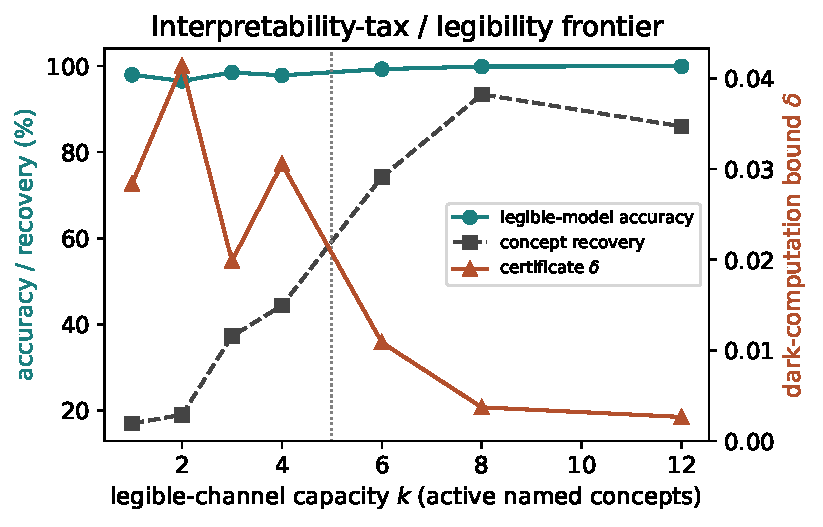
\includegraphics[width=\linewidth]{figures/tax_frontier.pdf}
\caption{The interpretability-tax / legibility frontier. As the legible channel's
capacity $k$ (active named concepts) grows past the task's true concept count (dotted
line), legible-model accuracy and concept recovery saturate while the certificate
$\delta$ collapses: once the channel can carry the task's concepts, legibility is nearly
free.}
\label{fig:tax}
\end{minipage}\hfill
\begin{minipage}[t]{0.49\textwidth}
\centering
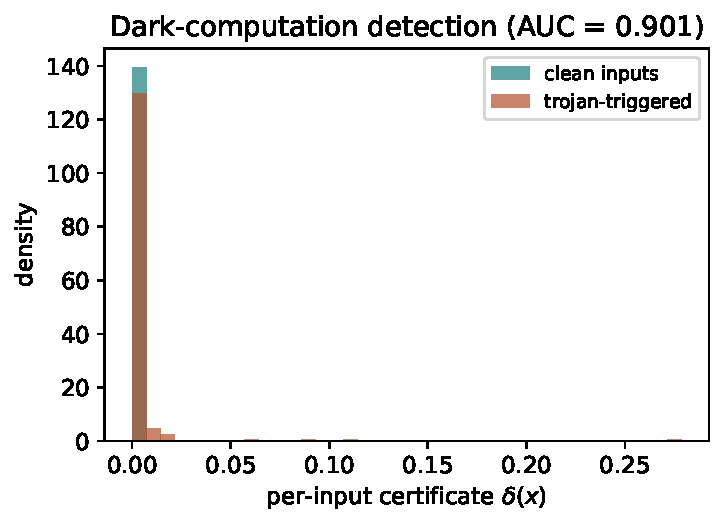
\includegraphics[width=\linewidth]{figures/trojan_detection.pdf}
\caption{Dark-computation detection. The per-input certificate $\delta(x)$ separates
clean inputs from backdoor-triggered inputs whose computation bypasses the named channel
(AUC \trojanAuc{}). A bypass cannot be both functional and hidden.}
\label{fig:trojan}
\end{minipage}
\end{figure}

\begin{figure}[t]
\centering
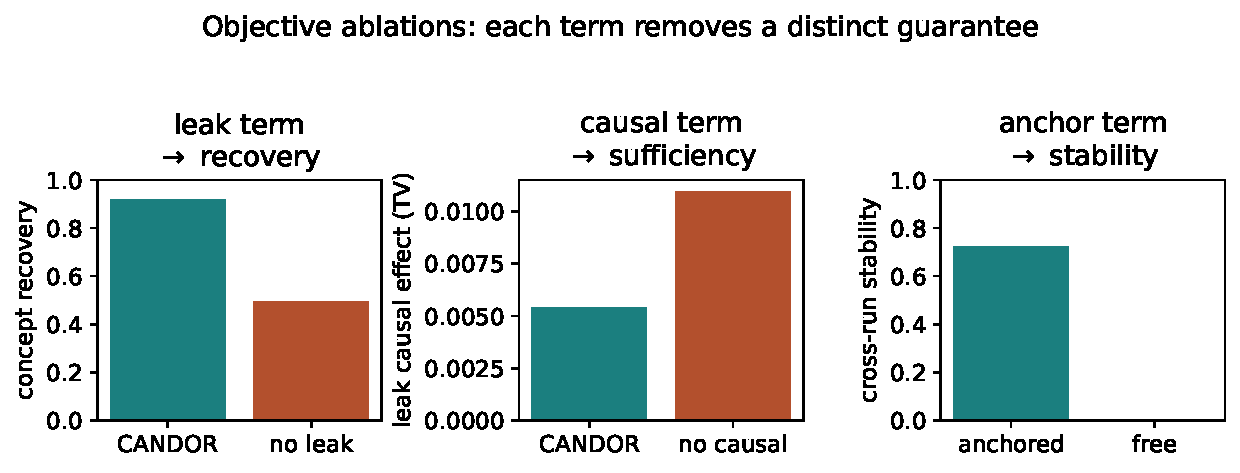
\includegraphics[width=0.92\textwidth]{figures/ablations.pdf}
\caption{Objective ablations: each term is load-bearing for a \emph{distinct} guarantee.
\textbf{Left:} the leak-energy term governs concept recovery (dropping it halves
recovery). \textbf{Centre:} the causal term governs causal sufficiency (dropping it
roughly doubles the leak's causal effect, mimicry without sufficiency). \textbf{Right:}
the anchoring term governs cross-run concept-identity stability (dropping it sends it to
zero). No single objective delivers all three; the conjunction does.}
\label{fig:abl}
\end{figure}

\section{Related work}
\label{sec:related}
We state precedents prominently: \emph{every component of CANDOR has antecedents}, and
the novelty is their conjunction operating jointly and at runtime.

\paragraph{Superposition and the legibility substrate.}
\citep{elhage2022superposition,elhage2021framework,olah2020zoomin,park2024linear,
hanni2024compsuperposition}. CANDOR inherits both the motivation for a sparse legible
basis and the completeness limit it concedes (Rem.~\ref{rem:incomplete}).

\paragraph{Sparse dictionaries and their crisis.}
\citep{bricken2023monosemanticity,cunningham2023sparse,templeton2024scaling,
gao2024scaling,rajamanoharan2024jumprelu,bussmann2025matryoshka,lieberum2024gemmascope,
chanin2024absorption,leask2025canonical,kantamneni2025useful}. CANDOR borrows the
sparse typed channel and the reconstruction (completeness) objective; it departs by
making the channel causal and certified rather than post-hoc, and by anchoring identity.

\paragraph{Transcoders, circuits, attribution.}
\citep{dunefsky2024transcoders,marks2024sparse,ameisen2025circuit,lindsey2025biology,
wang2022ioi,conmy2023acdc,syed2023eap,miller2024faithfulnessnotrobust}. CANDOR borrows
``the explanation is the forward pass'' and error-node accounting; it departs by routing
\emph{into} the trained forward pass and bounding the error-node mass at runtime.

\paragraph{Causal faithfulness as an objective.}
\citep{geiger2021causalabstractions,geiger2022iit,geiger2024das,wu2023boundlessdas,
chan2022causalscrubbing,geiger2025causalabstraction,makelov2023illusion}. This is
CANDOR's core borrowed engine. CANDOR generalises IIT from aligning a \emph{given}
causal variable to co-training a typed, persistent, \emph{complete} bottleneck plus a
runtime certificate; it does not invent training-time causal faithfulness.

\paragraph{By-construction interpretability and its leakage.}
\citep{koh2020concept,alvarezmelis2018senn,espinosa2022concept,chen2019thislooks,
bohle2022bcos,oord2017vqvae,hewitt2023backpack,rudin2019stop,mahinpei2021promises,
havasi2022addressing,locatello2019challenging}. CANDOR is a concept bottleneck hardened
with the guarantees this line proved necessary; \emph{leakage is dark computation under
another name}, and the certificate is what bounds it.

\paragraph{Certification, oversight, evaluation, governance.}
\citep{katz2017reluplex,zhang2018crown,xu2020autolirpa,przybysz2023verifying,
ignatiev2019abduction,christiano2021elk,roger2023measurement,lanham2023measuring,
chen2025reasoning,baker2025monitoring,korbak2025cot,jacovi2020faithfully,
karvonen2025saebench,amodei2025urgency,clymer2024safetycases,euaiact2024}. CANDOR
borrows the sound-over-approximation form and the safety-case framing, and supplies the
runtime certificate that monitoring and CoT approaches cannot. The runtime-certificate
stance also continues a line of \emph{certifying} runtime guardrails for deployed
models, but moves the certificate from the model's \emph{outputs} to the model's own
\emph{computation}.

\section{Limitations and honest scope}
\label{sec:limits}
\begin{itemize}[leftmargin=1.4em,itemsep=1pt]
\item \textbf{Scale, and the retrofit/by-construction gap.} Our positive evidence is on
synthetic ground-truth tasks and a one-layer Transformer, \emph{not} a frontier LLM; we
chose the regime where soundness can be \emph{checked}. On the real pretrained GPT-2
(\S\ref{sec:gpt2}) the certificate \emph{machinery} transfers, but a \emph{frozen} retrofit
does not favour CANDOR over a reconstruction-only SAE, because CANDOR's gains require the
model to reshape its computation through the channel, which only \emph{by-construction}
training provides. The single most important next experiment is therefore by-construction
training (or layer-wise fine-tuning) of a pretrained LLM with the bottleneck, followed by a
frontier-scale evaluation (SAEBench, RAVEL, MIB, and a real backdoor-detection
battery~\citep{karvonen2025saebench,huang2024ravel,mueller2025mib}); both are future work,
not present claims. Whether the favourable tax/legibility frontier persists at scale is the
central open empirical question.
\item \textbf{No completeness.} By Rem.~\ref{rem:incomplete} we do not and cannot claim
the certificate reaches zero on arbitrary computation; we claim it is sound, measured,
and trainable, and that a large $\delta$ is an honest abstention signal.
\item \textbf{``Certificate'' $\neq$ formal proof.} $\delta(x)$ is a sound \emph{per-input
measurement}, not a verified bound over all inputs. It is one-sided (cannot under-report
divergence for the inputs evaluated) but says nothing, on its own, about inputs not run.
A periodic exact certificate on a tractable channel fragment~\citep{przybysz2023verifying}
and a worst-case bound-propagation audit~\citep{xu2020autolirpa} are the natural
complements.
\item \textbf{Anchoring tension.} Anchoring injects inductive bias to stabilise identity;
pushed too hard it makes concepts the designer's labels rather than the model's. We report
where CANDOR sits via the cross-run stability number rather than assuming the best case.
\item \textbf{Concept placement.} On the planted task we place the concept layer where
the generative factors are linearly present; identifying such sites automatically in a
deep agent is unsolved, and computation that is irreducibly distributed across many
sites will show up as leak, not as a clean concept.
\end{itemize}

\section{Broader impact}
This work is about transparency and oversight of capable AI. A runtime, sound, checkable
bound on a model's non-legible computation is exactly the kind of artefact a safety case
for an autonomous agent needs~\citep{clymer2024safetycases,amodei2025urgency} and that
transparency regulation increasingly asks for~\citep{euaiact2024}. The same mechanism is
dual-use only in the weak sense that any interpretability tool is: it makes models easier
to understand, audit, and correct. The honest risk we flag is \emph{false assurance}:
treating a low $\delta$ on a test distribution as a guarantee off-distribution. We
therefore frame $\delta$ as a measurement with stated assumptions, demonstrate that it
\emph{rises} on bypassing computation rather than staying silent, and release everything
needed to recompute it.

\section{Conclusion}
Interpretability has been practised as archaeology: build an opaque artefact, then dig.
We have argued that the way toward interpretable AI systems is to stop digging, to make
legibility an architectural invariant and emit the audit at inference time. The Legible
Bottleneck is the single primitive that makes this possible: route a layer's computation
through a sparse, typed, anchored concept code, keep and \emph{measure} the unexplained
leak, and train the concepts to be causally sufficient. The resulting CANDOR
architecture certifies each of its decisions with a sound, re-checkable bound on its own
dark computation, recovers ground-truth concepts at near-zero tax, and surfaces a
channel-bypassing backdoor that no post-hoc method bounds. It is not a solution to
interpretable AI, and it does not claim completeness. It is a concrete, checkable
mechanism for turning interpretability from a description one hopes is true into an
invariant the model proves, one forward pass at a time.

\section*{Reproducibility statement}
Every number in this paper is machine-generated: \path{experiments/run_all.py}
(and \path{experiments/exp_gpt2.py} for \S\ref{sec:gpt2}) writes raw results to
\path{results/*.json}, \path{scripts/paper_numbers.py} converts them into the
macros used in the text (\path{paper/_numbers.tex}), and
\path{scripts/make_figures.py} renders the figures. No number is hand-entered, and
\texttt{make all} reproduces the paper end-to-end from a fresh checkout. All random
seeds are fixed in the experiment scripts (Appendix~\ref{app:details}); the experiments
run on commodity hardware (CPU is sufficient), and the GPT-2 experiment uses only the
publicly available GPT-2 small weights and a public text corpus. Code, the reference
implementation (\texttt{candorkit}), unit tests, and all measured results are available
under an MIT license at \url{https://github.com/AnwarDebes/candor}.

\bibliography{references}

\appendix

\section{Experimental details}
\label{app:details}
This appendix records every architecture, hyperparameter, and seed, as fixed in the
released code. Optimisation is plain Adam throughout; no learning-rate schedules,
weight decay, data augmentation, or early stopping are used anywhere. The anchoring
reference $\bar W$ is an exponential moving average of the decoder with momentum
$0.99$, updated once per step.

\subsection{Planted concepts (\S\ref{sec:planted})}
\textbf{Data.} $20{,}000$ samples; $K=\nConcepts$ independent Bernoulli concepts with
density $0.3$, mixed linearly into $\nIn$ dimensions with additive Gaussian noise
($\sigma=0.1$); the label counts the active concepts among a fixed relevant subset of
size $\nRelevant$ ($\nClasses$ classes); generation seed $0$; $80/20$ train/validation
split (seed $0$).

\textbf{Model.} CANDOR-MLP: the concept layer sits on a frozen, identity-initialised
embedding of the input; dictionary $m=\dictM$, $k=\topK$; task head with two hidden
layers of width $128$.

\textbf{Training.} \plantedSteps{} steps, Adam, learning rate $2\times10^{-3}$, batch
size $512$, seed $0$. Loss weights: $\alpha=0.5$ (legible task), $\beta=1.0$
(faithfulness), $\lambda=1.0$ (leak energy), $\mu=0.5$ (causal sufficiency),
$\gamma=10^{-2}$ (anchoring), plus an $L_1$ code penalty of $2\times10^{-3}$.

\textbf{Baseline.} An opaque MLP of matched shape (width $128$, two hidden layers)
trained for the same \plantedSteps{} steps (learning rate $2\times10^{-3}$, batch
$512$), followed by a post-hoc TopK SAE ($m=\dictM$, $k=\topK$) fitted to its
embedding for $2{,}000$ steps (Adam, learning rate $10^{-3}$, batch $1{,}024$, MSE
reconstruction, decoder columns renormalised each step).

\textbf{Causal tests.} Atoms are matched to generative concepts by Hungarian
assignment on absolute Pearson correlation. The \emph{necessity} test ablates (zeroes)
the atoms matched to the relevant concepts and compares the legible decision-flip rate
against ablating an equal number of irrelevant atoms. The \emph{directional} test
ablates one relevant concept's atom at a time, on the inputs where that concept is
active, and checks that the legible decision moves by exactly the amount the
ground-truth mechanism dictates (one class down, for the sum task), and symmetrically
that ablating an irrelevant concept's atom leaves the decision unchanged. Both tests
run on up to $1{,}500$ held-out validation inputs; neither intervention appears in the
training objective.

\textbf{Ablations.} Each ablation retrains from the same initialisation (seed $0$)
with one weight zeroed: no-faithfulness ($\beta=0$), no-leak ($\lambda=0$), no-causal
($\mu=0$), no-anchoring ($\gamma=0$); remaining weights $\beta=1.0$, $\lambda=1.0$,
$\mu=0.5$, $\gamma=10^{-2}$ as applicable, $L_1$ penalty $10^{-3}$.

\textbf{Frontier sweep (Fig.~\ref{fig:tax}).} The tax/legibility frontier retrains the
same architecture at channel capacities $k\in\{1,2,3,4,6,8,12\}$ for $1{,}600$ steps
each (learning rate $2\times10^{-3}$, batch $512$, seed $0$) with the default loss
weights ($\alpha=0.5$, $\beta=1.0$, $\lambda=0.3$, $\mu=0.3$, $\gamma=10^{-2}$, $L_1$
$10^{-3}$), on the same data and split as the main run.

\textbf{Stability protocol.} Three training runs (seeds $11$, $22$, $33$) per
condition; the \emph{anchored} condition uses anchoring weight $10^{-2}$ and a shared
dictionary initialisation (the anchor's reference point), the \emph{free} condition
uses no anchoring and per-seed initialisation; remaining weights at their defaults
($\alpha=0.5$, $\beta=1.0$, $\lambda=0.3$, $\mu=0.3$, $L_1$ $10^{-3}$). Reported
stability is the mean pairwise concept-identity agreement across runs.

\textbf{Backdoor (\S\ref{sec:trojan}).} $20{,}000$ samples with $K=\nConcepts$
concepts of which $3$ are relevant, density $0.3$, noise $0.1$; the base task is the
parity of the relevant concepts (binary). The trigger is a fixed unit direction in $4$
extra input dimensions (total input dimension $52$), disjoint from the concept mixing
directions by construction, added with magnitude $3.0$ against background noise
$\sigma=0.1$; it is planted in a nominal $5\%$ of inputs (measured \trojanRate\% of the
validation split) and flips the label. The model (same architecture) is trained with
the default loss weights for \plantedSteps{} steps; detection AUC uses the per-input
$\delta(x)$ as the score, with no access to trigger labels.

\subsection{Sequence task (\S\ref{sec:seq})}
\textbf{Data.} $12{,}000$ sequences of length \seqLen{} over a vocabulary of
\seqVocab{} tokens (generation seed $0$); the label is the maximum token
(\seqClasses{} classes); $85/15$ split (\seqTrain{} train / \seqTest{} test).

\textbf{Model.} One-layer Transformer: $d_{\mathrm{model}}=96$, $4$ attention heads,
MLP width $256$, with a Legible Bottleneck ($m=128$, $k=8$) on the MLP hidden state.

\textbf{Training.} $1{,}200$ steps, Adam, learning rate $10^{-3}$, batch size $256$,
seed $0$; loss weights $\alpha=0.5$, $\beta=1.0$, $\lambda=0.5$, $\mu=0.3$,
$\gamma=10^{-2}$, $L_1$ penalty $10^{-3}$; trained on CPU.

\subsection{GPT-2 retrofit (\S\ref{sec:gpt2})}
\textbf{Setup.} GPT-2 small (\gptParams{}M parameters, frozen throughout); a
transcoder-style Legible Bottleneck reads the MLP input and predicts the MLP output at
layer \gptLayer{} of \gptNLayer{}, spliced into the live model via a forward hook.
Corpus: the public TinyShakespeare text, tokenised with the GPT-2 tokeniser into
$1{,}400$ sequences of length $24$; $85/15$ split ($1{,}190$ train / \gptValSeqs{}
validation sequences).

\textbf{Channels.} Both channels use $m=\gptDictM$, $k=\gptTopK$, unit-norm decoder
columns, and identical training budgets: $250$ steps, Adam, learning rate
$2\times10^{-3}$, batch size $12$, seed $0$, on CPU. The \emph{SAE} channel minimises
normalised MSE reconstruction of the MLP output only. The \emph{CANDOR} channel adds
the behavioural faithfulness term (KL between the spliced legible model's next-token
distribution and the cached full-model distribution) and the causal-sufficiency term
(total variation against the leak-swapped splice), each with weight $1.0$.

\textbf{Metrics.} $\delta$ is the mean total-variation distance between the full and
legible-spliced next-token distributions on held-out text; the leak-swap effect is the
same quantity against the leak-swapped splice; unexplained variance is residual energy
over output energy; the loss-recovered fraction compares the legible splice's language
modelling loss against the full model and a zero-ablated MLP.

\subsection{Compute}
All experiments run on a single commodity machine; no data-centre resources are used.
Each \texttt{results/*.json} file records the device and wall-clock time of the run
that produced it.

\end{document}
